\documentclass[alternative-exam.tex]{subfiles}
\begin{document}

\chapter{Een ei bakken}
\section{Vraag}
Als student krijg je tijdens het werken wel eens zin in spek met eieren. Als luie student vind je het al een opgave om naar de keuken te gaan om het eitje te bakken. Voor je vertrekt naar de keuken wil je al precies weten welke stappen je moet ondernemen, zodat je zeker niet teveel moeite doet. Met het STRIPS planning algoritme kan je dit probleem oplossen.

\subsection{Begin- en Eindsituaties}
\begin{figure}[H]
\centering
\begin{tabular}{|c|c|}
    \multicolumn{2}{c}{I}\\
    \hline
    if & -\\
    \hline
    add & In(Kamer)\\
        & Vrij(Pan)\\
    \hline
    del & -\\
    \hline
\end{tabular}
\begin{tabular}{|c|c|}
    \multicolumn{2}{c}{F}\\
    \hline
    if & In(Kamer)\\
    & heeft(Maaltijd)\\
    \hline
    add & -\\
    \hline
    del & -\\
    \hline
\end{tabular}
\caption{begin- en eindtoestand}
\label{ienf}
\end{figure}
Figuur \ref{ienf}, toont de begintoestand en de gewenste eindtoestand. In de begintoestand zit de student aan zijn bureau in zijn kamer en heeft hij honger. In de eindtoestand zit de student weer aan zijn bureau en heeft hij een bord met gebakken spek en eieren.
\subsection{Acties}
Het hele proces kan beschreven worden een door aantal acties die de student kan ondernemen.
\begin{itemize}
\item
De student kan naar de keuken wandelen en terug. In figuur \ref{keuken} staan de overeenkomstige acties beschreven.
\begin{figure}[H]
\centering
\begin{tabular}{|c|c|}
    \multicolumn{2}{c}{H}\\
    \hline
    if & In(Kamer)\\
    \hline
    add & In(Keuken)\\
    \hline
    del & In(Kamer)\\
    \hline
\end{tabular}
\begin{tabular}{|c|c|}
    \multicolumn{2}{c}{T}\\
    \hline
    if & In(Keuken)\\
    \hline
    add & In(Kamer)\\
    \hline
    del & In(Keuken)\\
    \hline
\end{tabular}
\caption{van en naar de keuken wandelen}
\label{keuken}
\end{figure}
\item 
In de keuken kan de student koken en alle overeenkomstige acties daarvoor staan beschreven in figuur \ref{koken}.
\begin{figure}[H]
\centering
\begin{tabular}{|c|c|}
    \multicolumn{2}{c}{NeemEi (NE)}\\
    \hline
    if & In(Keuken)\\
    \hline
    add & Heeft(RauwEi)\\
    \hline
    del & -\\
    \hline
\end{tabular}
\begin{tabular}{|c|c|}
    \multicolumn{2}{c}{NaamSpek (NS)}\\
    \hline
    if & In(Keuken)\\
    \hline
    add & Heeft(RauwSpek)\\
    \hline
    del & -\\
    \hline
\end{tabular}
\\\vspace{0.25cm}
\begin{tabular}{|c|c|}
    \multicolumn{2}{c}{BakEi (BE)}\\
    \hline
    if & In(Keuken)\\
    & Vrij(Pan)\\
    & Heeft(RauwEi)\\
    \hline
    add & Heeft(EiKlaar)\\
    \hline
    del & Heeft(RauwEi)\\
    \hline
\end{tabular}
\begin{tabular}{|c|c|}
    \multicolumn{2}{c}{BakSpek (BS)}\\
    \hline
    if & In(Keuken)\\
    & Vrij(Pan)\\
    & Heeft(RauwSpek)\\
    \hline
    add & Bakt(Spek)\\
    \hline
    del & Heeft(RauwSpek)\\
    & vrij(Pan)\\
    \hline
\end{tabular}
\\\vspace{0.25cm}
\begin{tabular}{|c|c|}
    \multicolumn{2}{c}{DraaiSpekOm (DSO)}\\
    \hline
    if & In(Keuken)\\
    & Bakt(Spek)\\
    \hline
    add & Heeft(SpekKlaar)\\
    & Vrij(Pan)\\
    \hline
    del & Bakt(Spek)\\
    \hline
\end{tabular}
\begin{tabular}{|c|c|}
    \multicolumn{2}{c}{LegOpBord(LOB)}\\
    \hline
    if & In(Keuken)\\
    & Heeft(SpekKlaar)\\
    & Heeft(EiKlaar)\\
    \hline
    add & Heeft(Maaltijd)\\
    \hline
    del & Heeft(SpekKlaar)\\
    & Heeft(EiKlaar)\\
    \hline
\end{tabular}
\caption{koken}
\label{koken}
\end{figure}
\end{itemize}

\section{Modeloplossing}
\subsection{Establishes/Threathens-graaf}
\begin{figure}[p]
\centering
\caption{Establishes/Threathens-graaf}
\label{strips_1}
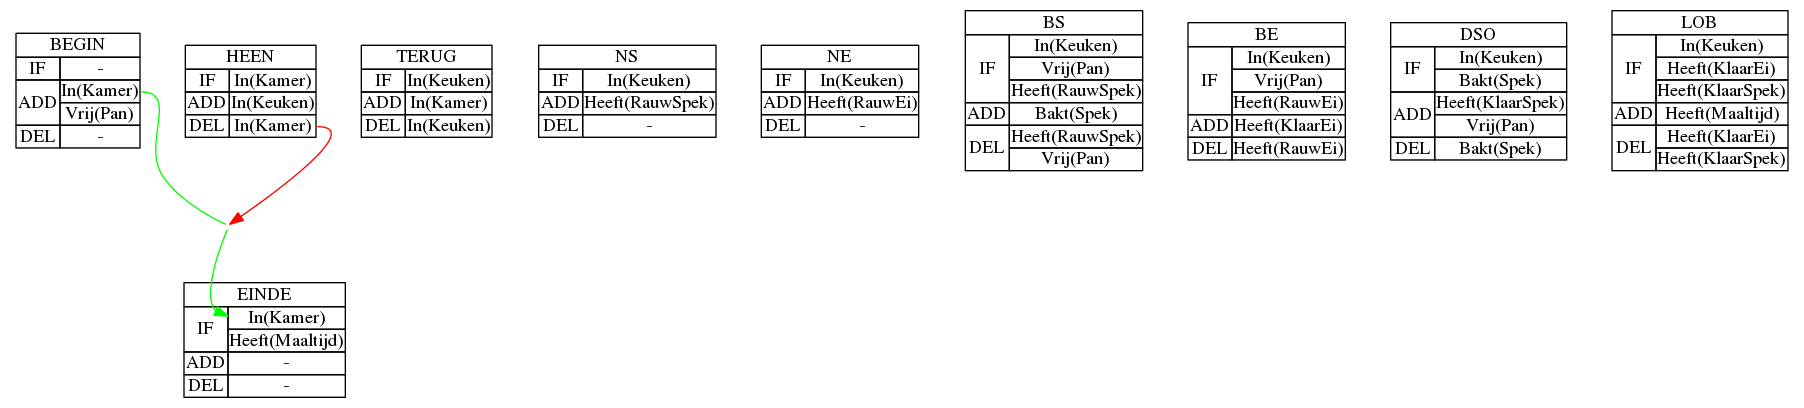
\includegraphics[scale=0.3]{resources/graphs/strips_1.png}
\end{figure}

\subsection{Before-graaf}


\end{document}